\documentclass{article}

\usepackage{graphicx}
\usepackage[margin=2cm,a4paper]{geometry}
\usepackage{tcolorbox}
\tcbuselibrary{listings,skins}
\usepackage{listings}
\lstset{
  language=bash,
  basicstyle=\small\ttfamily,
  columns=flexible,
  breaklines=true,
  showstringspaces=false,
  frame=single
}

\begin{document}

\title{Building IaaS infrastructures on the AWS Cloud}
\author{Saul Pierotti}
\date{\today}

\maketitle

\begin{abstract}
The abstract text goes here.
\end{abstract}

\section{General Description of the Infrastructure}
The demostrative infrastructure described in this project consists of an HTCondor cluster of three nodes.
One node is configured as Master Node, while 2 nodes are configured as Worker Nodes.
The infrastructure can be easily expanded by replicating the Worker Node instances.
The Master Node was not used also as a Worker Node since the performance benefits and cost savings would be marginal.
This was done also to avoid overloading the Master Node, on which the entire cluster depends.
A shared storage space directly attached to the Master Node but available to all the Worker Nodes was also implemented using the distributed file system NFS.

\section{Initialization of the instances on the AWS Cloud}
Worker Nodes and the Master Node were both built on the same base instance configuration.
The \texttt{t2.medium} instance type was used with a 50 Gb SSD as root storage.
The operating system choosen is Ubuntu Server 18.04.4 LTS.
The Master Node and the Worker Nodes were all instatiated in the same availability zone (\texttt{us-east-1a}), so that they would be able to communicate through private IPv4 adresses.
The security group for the instances was configured as follows:

\begin{figure}[!h]
	\center
	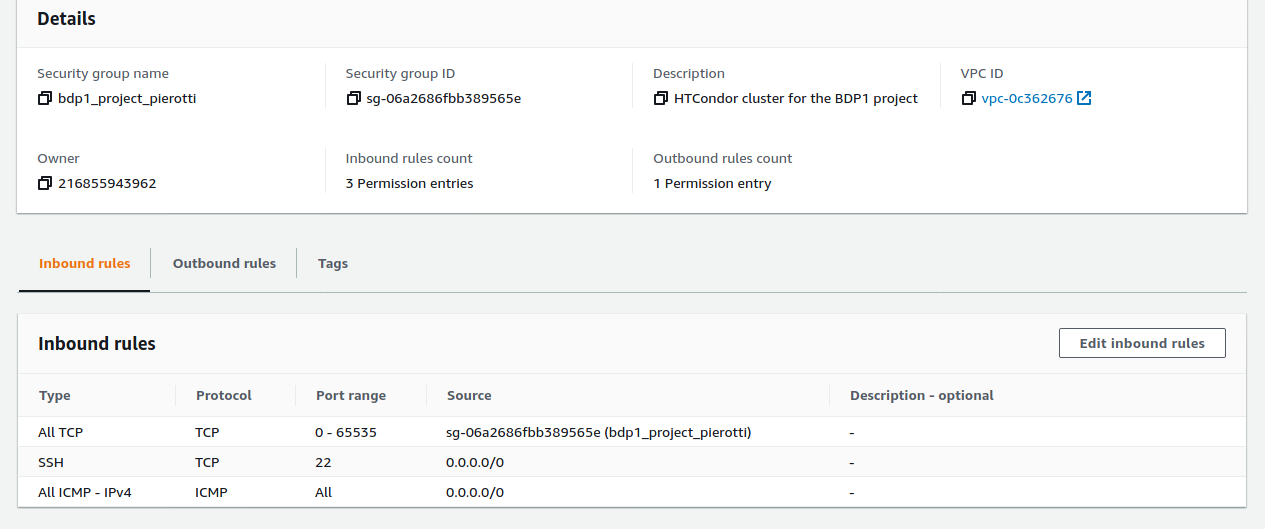
\includegraphics[width=\textwidth]{./images/security-group.png}
\end{figure}

All the TCP ports were opened to the other members of the same security group since HTCondor deamons use a dynamically assigned port.
The TCP ports were also needed for the setup of a shared NFS volume.
ICMP ports were opened for accepting incoming \texttt{ping} requests for testing purposes.
TCP port 22 was opened for allowing remote control of the machines via \texttt{ssh}.

\section{Configuration of the Master Node}
The PS1 prompt of the Master Node was changed so to make the node easily identifiable from the command line.

\begin{figure}[!h]
	\center
	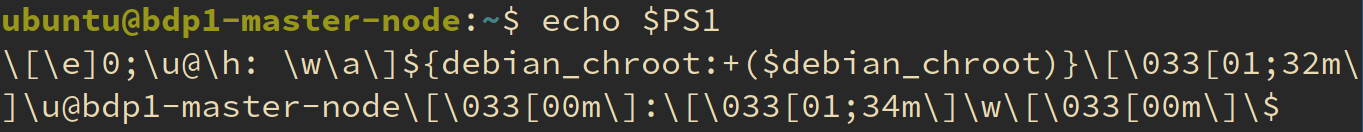
\includegraphics[width=\textwidth]{./images/master-ps1.png}
\end{figure}
\pagebreak

HTCondor was then installed with the following commands:

\begin{lstlisting}
sudo su
wget -qO - https://research.cs.wisc.edu/htcondor/ubuntu/HTCondor-Release.gpg.key | apt-key add - # import the gpg key of HTCondor
echo "deb http://research.cs.wisc.edu/htcondor/ubuntu/8.8/bionic bionic contrib" >> /etc/apt/sources.list # add the repository
echo "deb-src http://research.cs.wisc.edu/htcondor/ubuntu/8.8/bionic bionic contrib" >> /etc/apt/sources.list
apt update
apt install htcondor
systemctl start condor # start and enable the condor service
systemctl enable condor
\end{lstlisting}

The correct proceeding of the installation and the start of the \texttt{condor} service where checked with the following commands:

\begin{figure}[!h]
	\center
	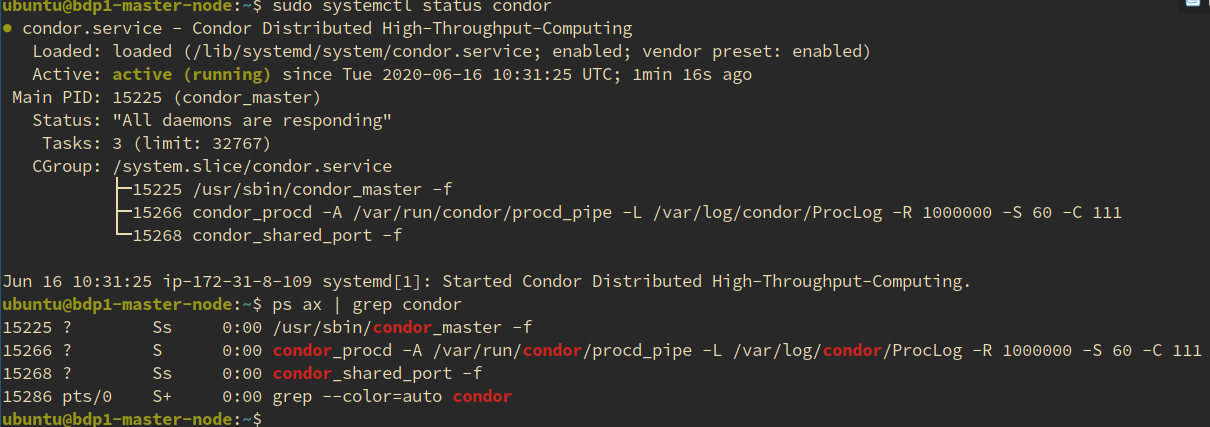
\includegraphics[width=\textwidth]{./images/condor_installed.png}
\end{figure}

The following lines where appended at the end of the main HTCondor configuration file, located at\\
\texttt{/etc/condor/condor\_config}:

\begin{lstlisting}
# Master Node IP
CONDOR_HOST = <Master_Node_private_IP>

# Master Node config 
DAEMON_LIST = COLLECTOR, MASTER, NEGOTIATOR, STARTD
\end{lstlisting}

Finally, the \texttt{condor} service was restarted with the following command:

\begin{lstlisting}
sudo systemctl restart condor
\end{lstlisting}

The NFS server was then implemented in the Master Node.
A new 100 Gb standard magnetic volume was created from the AWS interface and attached to the Master Node.
From the server, a primary partiton was initialized on the volume using \texttt{fdisk} and an \texttt{Ext4} file system was created onto it using \texttt{mkfs.ext4}.
The file \texttt{/etc/fstab} of the Master Node was modified so that the machine would mount the volume automatically at boot under the newly created directory \texttt{/data}.
The following line was appended to \texttt{/etc/fstab}:

\begin{lstlisting}
</new_volume/partiton>              /data    ext4   defaults                0 0
\end{lstlisting}

The following commands were then issued, so to install the appropriate packages:

\begin{lstlisting}
sudo apt install nfs-kernel-server
\end{lstlisting}

The following line was appended to the NFS configuration file \texttt{/etc/exports}:

\begin{lstlisting}
/data 172.31.0.0/16(rw,sync,no_wdelay)
\end{lstlisting}

Finally, the owner and group of the shared folder was changed to \texttt{nobody:nogroup} and the permission of the folder were edited so to grant unlimited access to it:

\begin{lstlisting}
sudo chown nobody:nogroup /data
sudo chmod 777 /data
\end{lstlisting}

The \texttt{/data} folder was so made available to all the Worker Nodes on the address range \texttt{172.31.0.0/16}.
This configuration does not pose a security risk since the the Master Node and Worker Nodes machines belong to a Virtual Private Cloud (VPC), and so only machines instatiated on it will be able to access the volume.
Moreover, this configuration grants immediately access to the volume to newly instantiated Worker Nodes.
A mock file was created on the \texttt{/data} folder so to be able to recognize it when mounted.

\begin{lstlisting}
touch /data/this_is_a_shared_NFS_volume
\end{lstlisting}

\section{Configuration of the Worker Nodes}
A virtual machine identical to the one used for the Master Node was instantiated.
The PS1 prompt of this first Worker Node was changed so to make the node easily identifiable from the command line.

\begin{figure}[!h]
	\center
	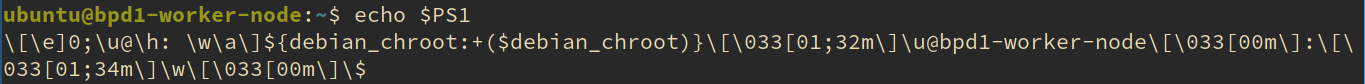
\includegraphics[width=\textwidth]{./images/worker-ps1.png}
\end{figure}

HTCondor was installed in this system with the same procedure used for the Master Node.
Only the \texttt{/etc/condor/condor\_config} file was configured differently, by appending the following lines to it:

\begin{lstlisting}
# Master Node IP
CONDOR_HOST = <Master_Node_private_IP>

# Worker Node config
DAEMON_LIST = MASTER, STARTD

HOSTALLOW_READ = *
HOSTALLOW_WRITE = *
HOSTALLOW_ADMINISTRATOR = *
\end{lstlisting}

On the Worker Node access to the shared NFS volume was then set up.
The following command was issued to install the required packages and enable the respective services:

\begin{lstlisting}
sudo apt install nfs-common
sudo systemctl start nfs-server
sudo systemctl enable nfs-server
\end{lstlisting}

A new directory was then created at \texttt{/data} using the \texttt{mkdir} command.
The \texttt{/etc/fstab} file was edited by appending the following line, so that the shared volume would be automatically mounted at boot under the directory \texttt{/data}:

\begin{lstlisting}
<Master_Node_private_IP>:/data      /data    nfs    defaults                0 0
\end{lstlisting}

It was then verified that the shared volume was accessible from the Worker Node.

\begin{figure}[!h]
	\center
	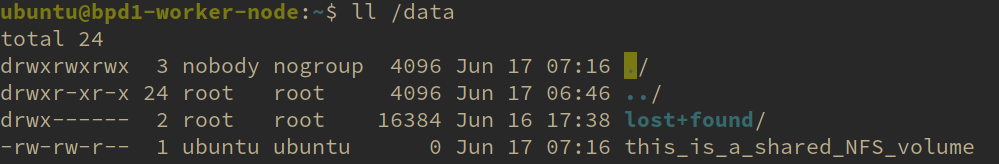
\includegraphics[width=\textwidth]{./images/nfs_works.png}
\end{figure}

An image of the virtual machine was taken through the AWS interface.
In this way, the Worker Nodes would be easily replicable when more computational power is needed by instaciating new virtual machines from the image, without the need for manual configuration.

\section{Submission of a test job to the HTCondor cluster}
For demostrating the use of the newly created cluster, a new Worker Node was instanciated from the Worker Node image, so that the cluster would contain the Master Node and 2 Worker Nodes.

A new volume was created from the AWS interface from a snapshot containing test data for the BDP1 course (\texttt{snap-09ee52d8038fb8094}, BDP1\_2020).
This snapshot contains biological data to be used for testing the infrastructure.
It contains NGS reads from 3 different patients.
Each patient has a folder with around 500 fasta files, with 1000 reads each.
This data will be used for testing the infrastructure.
This new volume was mounted on the Master Node under \texttt{/data}, substituting the empty volume used before.
The \texttt{/etc/fstab} file was update accordingly and the \texttt{nfs-server} service restarted.
It was then tested that the new volume was accessible from the Worker Nodes.

\begin{figure}[!h]
	\center
	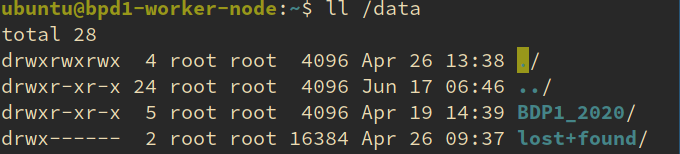
\includegraphics[width=.8\textwidth]{./images/nfs_bdp_works.png}
\end{figure}

The test job consisted in alligning 1 fasta file from 1 patient to the human genome build hg19, also stored on the shared volume.
The BWA alignment tool was used for the scope.
This tool takes advantage of indexing the genome for speeding up the alignment of low-divergent reads to it.
The index for the hg19 build was already present in the volume snapshot, so there was no need to create it from scratch.
The test reads were copied from the shared volume to the home folder of the Master Node.
The test job file \texttt{alignment\_test.job} was created, with the following content:

\begin{lstlisting}
####################################################
################### Alignment Test #################
####################################################


########### The program that will be executed #######

Executable = alignment_test.py

############ Input Sandbox  #########################

Input      = read_1.fa

transfer_input_files = read_1.fa

###### Output Sandbox ###############################

Log        = condor.log
# will contain condor log

Output     = condor.out
# will contain the standard output

Error      = condor.error
# will contain the standard error

############## condor control variables #############

should_transfer_files = YES
when_to_transfer_output = ON_EXIT

Universe = vanilla

#####################################################
Queue

\end{lstlisting}
\pagebreak

The script \texttt{alignment\_test.py} was the following:

\begin{lstlisting}
#!/usr/bin/python
import sys,os
from timeit import default_timer as timer

start = timer()
dbpath = "/data/BDP1_2020/hg19/"
dbname = "hg19bwaidx"
basename = "read_1"
queryname = basename+".fa"
out_name = basename 
md5file = out_name+".md5"

# install bwa
os.system('sudo apt install -y bwa')

command = "bwa aln -t 1 " + dbpath + dbname + " " + queryname + " > " + out_name + ".sai"
print "launching command: " , command
os.system(command)

command = "bwa samse -n 10 " + dbpath + dbname + " " + out_name + ".sai " + queryname + " > " + out_name + ".sam"
print "launching command: " , command
os.system(command)

# Checksums
print "Creating md5sums"
os.system("md5sum " + out_name + ".sam " + " > " + md5file)

print "gzipping out text file"
command = "gzip " + out_name + ".sam"
print "launching command: " , command
os.system(command)

# Transfer files to shared volume
gzipfile = out_name + '.sam.gz'
os.system('mv '+ gzipfile + ' /data/outputs/'+ gzipfile)
os.system('mv '+ md5file + ' /data/outputs/'+ md5file)

execution_time = timer() - start

print 'Total execution time: ' + str(execution_time)
print "exiting"

exit(0)
\end{lstlisting}

\section{Data Management Model}
The general model followed would be that of transferring the executables and the read file using the HTCondor Input Sandbox.
This is because those files are generally small and their transfer will not overload the Master Node.
In addition, this setup allows flexibility in choosing the application to be used and the input data.
On the contrary, the large hg19 genome and index files will be made availabe to the Worker Nodes through the shared NFS volume.
The Output Sandbox will contain the condor log, the standard output and the standard error.
The aligned reads will instead be compressed and put in the shared volume, so to avoid moving large data on the Output Sandbox.

\subsection{Creation of a Container Image for the Application}
A containerized version of the BWA application was built using \texttt{docker}.
A container image for the BWA application is already available on DockerHub (\texttt{biocontainers/bwa}), but for educational purposes a new image was built from scratch.
The Ubuntu 18.04.4 LTS Linux docker image was used as a base, and the following Dockerfile was created.

\begin{lstlistings}

\end{lstlistings}

\end{document}
